\documentclass[12pt]{article}
\usepackage{float}
% Packages for formatting
\usepackage{graphicx}    % For including images
\usepackage{fancyhdr}    % For custom headers and footers
\usepackage{geometry}    % For setting page margins
\usepackage{amsmath}     % For advanced mathematical formatting
\usepackage{hyperref}    % For hyperlinks
\usepackage{float}
\usepackage{verbatim}

% Page margins
\geometry{
    a4paper,
    left=1in,
    right=1in,
    top=1in,
    bottom=1in
}

% Header and Footer settings
\pagestyle{fancy}
\fancyhf{} % Clear all header and footer fields
\fancyhead[L]{\textbf{OS LAB TASK 8}}         % Left header
\fancyhead[R]{\textbf{FAST NUCES}}     % Right header
\fancyfoot[C]{\thepage}                % Center footer with page number

% Title Information
\title{
    \vspace{-2cm} % Adjust vertical spacing
    \LARGE{\textbf{Operating Systems Lab Report}} \\
    \vspace{0.5cm}
    \Huge{Muhammad Shafeen} \\
    \Large{Student ID: 22P-9278}
}
\date{October 11, 2024} % No date

\begin{document}

\maketitle
\thispagestyle{fancy} % Apply the fancy header to the title page

\section*{Lab 8: Operating Systems}
\subsection{Open 2 Terminals}
Opening two terminals checking the process id and then 
\begin{figure}[H]
    \centering
    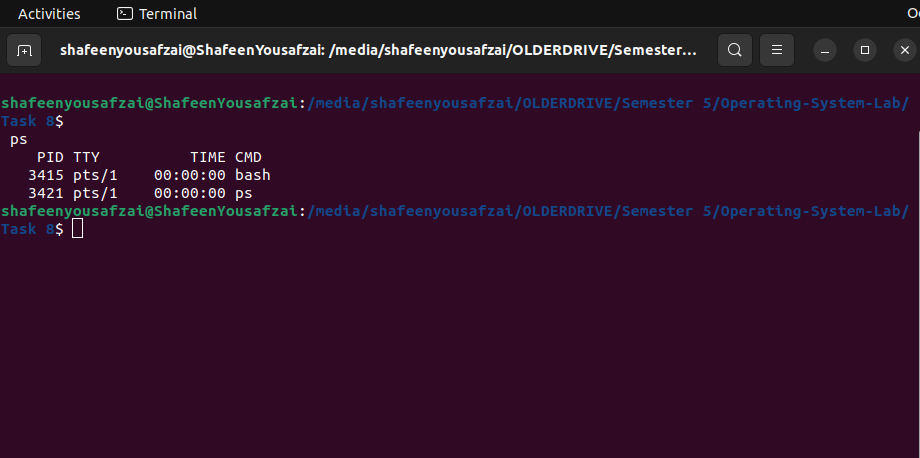
\includegraphics[width=0.8\textwidth]{Screenshot from 2024-10-11 08-17-18.png}
    \caption{Checking the process id by using PS}
    \label{fig:enter-label}
\end{figure}

\begin{figure}[H]
    \centering
    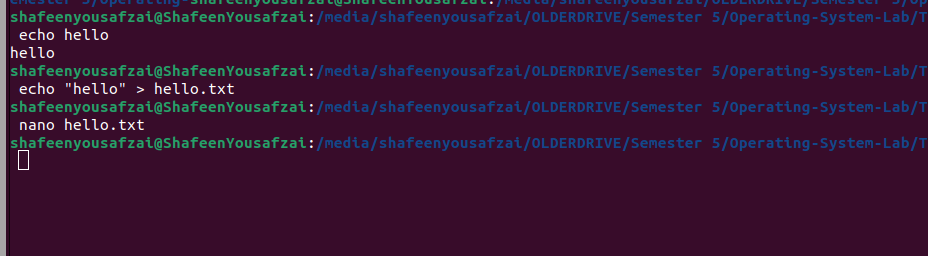
\includegraphics[width=0.8\textwidth]{Screenshot from 2024-10-11 08-17-34.png}
    \caption{Outputting hello on temrinal using cat >}
    \label{fig:enter-label}
\end{figure}

\begin{figure}[H]
    \centering
    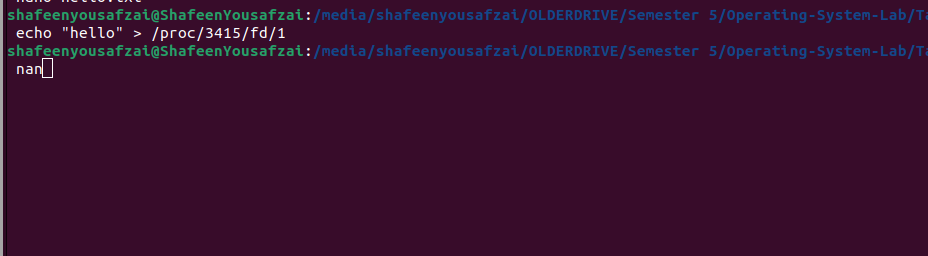
\includegraphics[width=0.8\textwidth]{Screenshot from 2024-10-11 08-19-57.png}
    \caption{Outputting hello on the proces id termianl}
    \label{fig:enter-label}
\end{figure}

\begin{figure}[H]
    \centering
    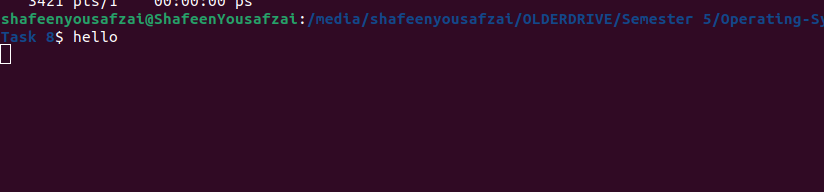
\includegraphics[width=0.8\textwidth]{Screenshot from 2024-10-11 08-20-01.png}
    \caption{Outputting hello on temrinal using cat >}
    \label{fig:enter-label}
\end{figure}

\begin{figure}[H]
    \centering
    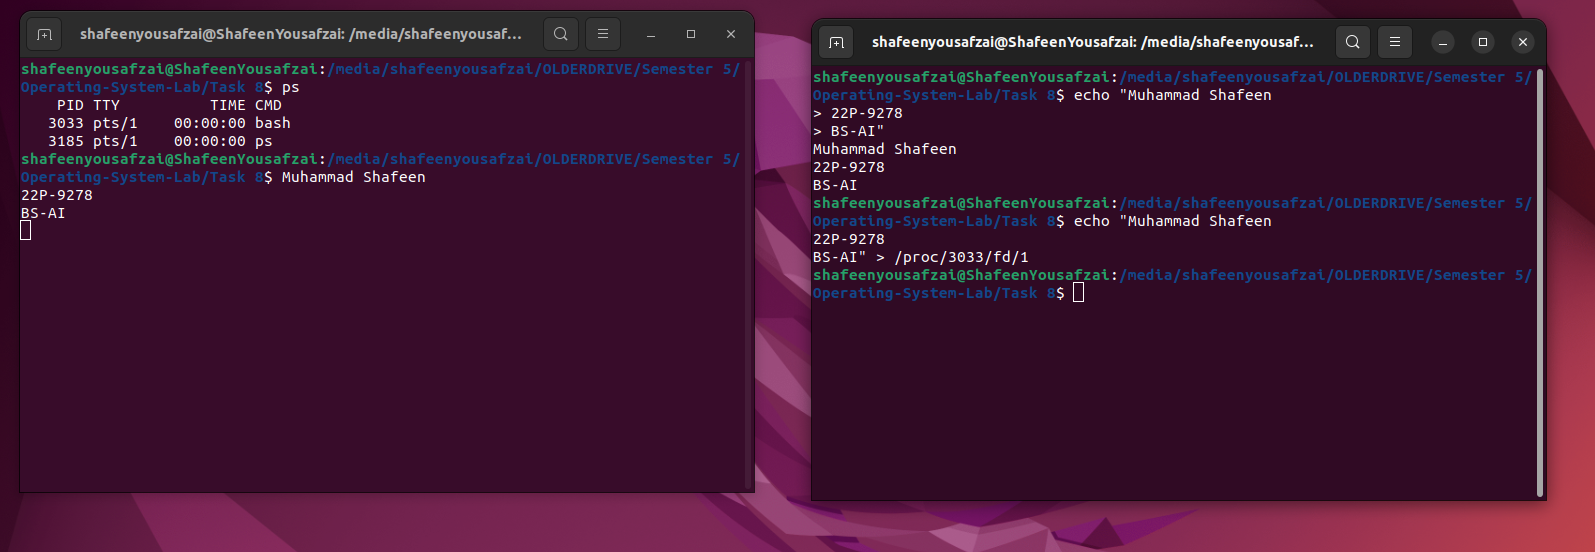
\includegraphics[width=0.8\textwidth]{Screenshot from 2024-10-11 08-23-49.png}
    \caption{Outputting Name,Roll,section}
    \label{fig:enter-label}
\end{figure}

\subsection{Run code and check file size}
\begin{verbatim}
    #include <fcntl.h>
#include <stdio.h>
#include <sys/stat.h>
#include <sys/types.h>
#include <unistd.h>
int main(int argc, char* argv[])
{
char *path = argv[1];
int fd = open(path, O_WRONLY | O_EXCL |
O_CREAT);
if (fd == -1)
{
printf("Error: File not Created\n");
return 1;
}
return 0;
}
\end{verbatim}
\begin{figure}[H]
    \centering
    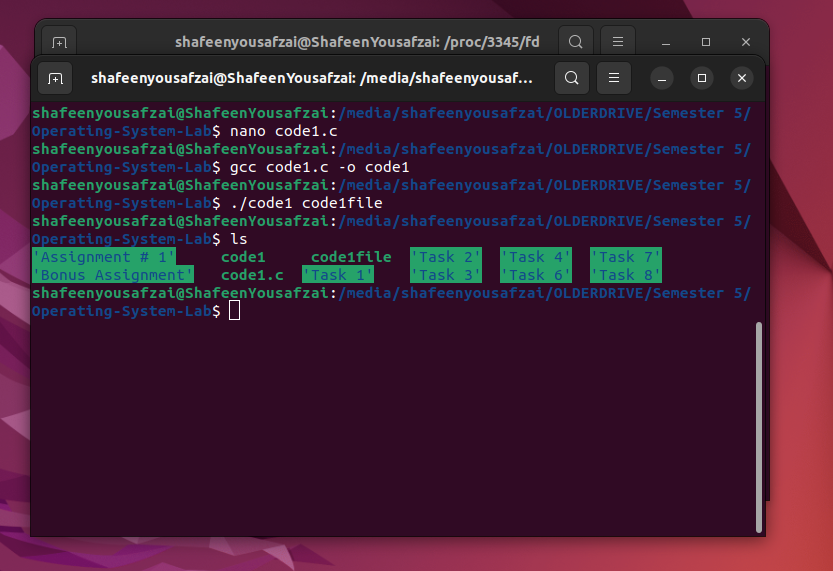
\includegraphics[width=0.8\textwidth]{Screenshot from 2024-10-11 08-38-50.png}
    \caption{Outputting the output of file and creating a file}
    \label{fig:enter-label}
\end{figure}

\subsection{Question}
Question What is the size of the file? Why
is it this size?
\subsection{Answer:}
The size of the process is 0 bytes becasue whenever a new file is created it takes 0 bytes of storage

\subsection{Question}
Check what the open() function return> 
\subsection{Answer:}
An exit code of 0 indicates success while a non-zero exit code
       indicates failure. The following failure codes can be returned:

       1
           Error in command line syntax.

       2
           One of the files passed on the command line did not exist.

       3
           A required tool could not be found.

       4
           The action failed.

\subsection{Close a File}
\begin{verbatim}
    #include <fcntl.h>
#include <stdio.h>
#include <sys/stat.h>
#include <sys/types.h>
#include <unistd.h>
int main(int argc, char* argv[])
{
if (argc != 2)
{
printf("Error: Run like this: ");
printf("%6s name-of-new-file\n", argv[0]);
return 1;
}
char *path = argv[1];
int i = 0;
while(i<2)
{
int fd = open(path, O_WRONLY | O_CREAT);
printf("Created! Descriptor is %d\n", fd);
close(fd);
i++;
}
return 0;
}
\end{verbatim}
\subsection{run without closing file}
\begin{verbatim}
    #include <fcntl.h>
#include <stdio.h>
#include <sys/stat.h>
#include <sys/types.h>
#include <unistd.h>
int main(int argc, char* argv[])
{
if (argc != 2)
{
printf("Error: Run like this: ");
printf("%6s name-of-new-file\n", argv[0]);
return 1;
}
char *path = argv[1];
int i = 0;
while(i<2)
{
int fd = open(path, O_WRONLY | O_CREAT);
printf("Created! Descriptor is %d\n", fd);
i++;
}
return 0;
}
\end{verbatim}
        \begin{figure}
            \centering
            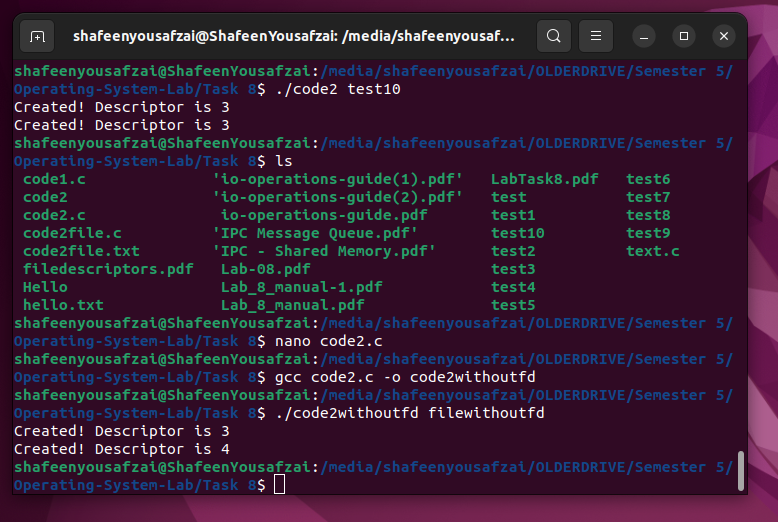
\includegraphics[width=0.8\textwidth]{image.png}
            \caption{Running the code without fd(close)}
            \label{fig:enter-label}
        \end{figure}
\subsection{Question : }
Writing to a file is done using the write call.
To write, we should obviously open a file first.
\subsection{Answer :}
we are getting 3 because one file is being run and we get a 4 because we did not close the file 
created before with a return descriptor of 3 .

\subsection{Writing to a file}
\begin{verbatim}
    #include <fcntl.h>
#include <stdio.h>
#include <string.h>
#include <sys/stat.h>
#include <sys/types.h>
#include <time.h>
#include <unistd.h>
char* get_timeStamp()
{
time_t now = time(NULL);
return asctime(localtime(&now));
}
int main(int argc, char* argv[])
{
char *filename = argv[1];
char *timeStamp = get_timeStamp();
int fd = open(filename, O_WRONLY |
O_APPEND |
O_CREAT, 0666);
size_t length = strlen(timeStamp);
write(fd, timeStamp, length);
close(fd);
return 0;
}

\end{verbatim}
\begin{figure}[H]
    \centering
    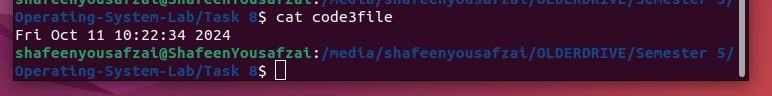
\includegraphics[width=0.8\textwidth]{1.png}
    \caption{Output of the code. print the output}
    \label{fig:enter-label}
\end{figure}
\subsection{Question : }
What is 0666 that is specified in the open()
call? What does it mean?
\subsection{Answer : }
0666 is the file permission mode in octal notation. It means the file will be
created with read and write permissions for the owner, group, and others.

\subsection{Question : }
What is O\_APPEND doing in the same call?
Run the program again and check its output.
\subsection{Answer : }
O\_APPEND flag ensures that the data is appended to
the end of the file. If you run the program multiple times, you’ll see multiple
timestamps in the file, one after another.

\subsection{Question : }
Modify the following line in the code and then compile and run the pro-
gram and check its output. What has happened? From: size\_t length =
strlen(timeStamp); To: size\_t length = strlen(timeStamp)-5
\subsection{Answer :}
By
reducing the length by 5, you’re truncating the last 5 characters of the times-
tamp. This will likely cut off the year and newline character from the timestamp
in the file.
\begin{figure}
    \centering
    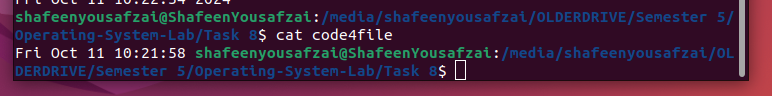
\includegraphics[width=0.8\textwidth]{2.png}
    \caption{Out of the file with -5 timestamp}
    \label{fig:enter-label}
\end{figure}

\begin{verbatim}
    #include <stdio.h>
#include <sys/stat.h>
#include <sys/types.h>
#include <unistd.h>
int main(int argc, char* argv[])
{
if (argc != 2)
{
printf("Error: Run like this: ");
printf("%6s name-of-existing-file\n",
argv[0]);
return 1;
}
char *path = argv[1];
int fd = open(path, O_RDONLY);
if (fd == -1)
{
printf("File does not exist\n");
return 1;
}
char buffer[200];
read(fd, buffer, sizeof(buffer)-1);
printf("Contents of File are:\n");
printf("%s\n", buffer);
close(fd);
return 0;
}

\end{verbatim}
\begin{figure}[H]
    \centering
    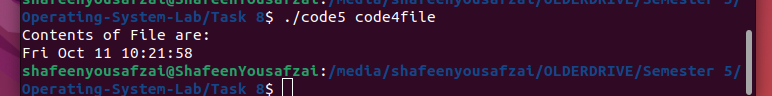
\includegraphics[width=0.9\textwidth]{3.png}
    \caption{Output of the last code file}
    \label{fig:enter-label}
\end{figure}
\end{document}